\def\autofocus{
    Từ vấn đề tồn đọng của phương pháp chuẩn bị dữ liệu SNIPER, mô hình AutoFocus \cite{najibi2019autofocus} đã ra đời nhằm tăng tốc quá trình dự đoán của mô hình object detection.
    AutoFocus hướng đến việc loại bỏ những pixel dư thừa mà mô hình phải xử lý trong quá trình dự đoán nhưng vẫn giữ được ý tưởng về việc sử dụng Image Pyramids.
    Mô hình AutoFocus được thiết kế nhằm dự đoán những khu vực đáng chú ý ở trên ảnh và loại bỏ những khu vực khả năng cao không chứa đối tượng ở những kích thước ảnh lớn hơn.
    Từ đó, tiết kiệm được rất nhiều chi phí tính toán trong quá trình predict của mô hình.

    \noindent
    \textbf{\textit{Kiến trúc tổng quá của mô hình AutoFocus}} \\
    Mô hình AutoFocus gồm hai nhánh: \\
    - Nhánh Focus (cụ thể gọi là Nhánh Focus Pixel Prediction) là nhánh mô hình giúp xác định được khu vực đáng chú ý trên ảnh để zoom to hơn, đồng thời loại bỏ các khu vực khả năng cao không chứa đối tượng. \\
    - Nhánh Detection là nhánh giúp mô hình định vị chính xác bounding box của từng đối tượng.
    Trong nghiên cứu, nhóm tác giả sử dụng mô hình Faster R-CNN \cite{ren2015faster} làm cơ sở cho nhánh Detection.

    \begin{figure}[H]
        \centering
        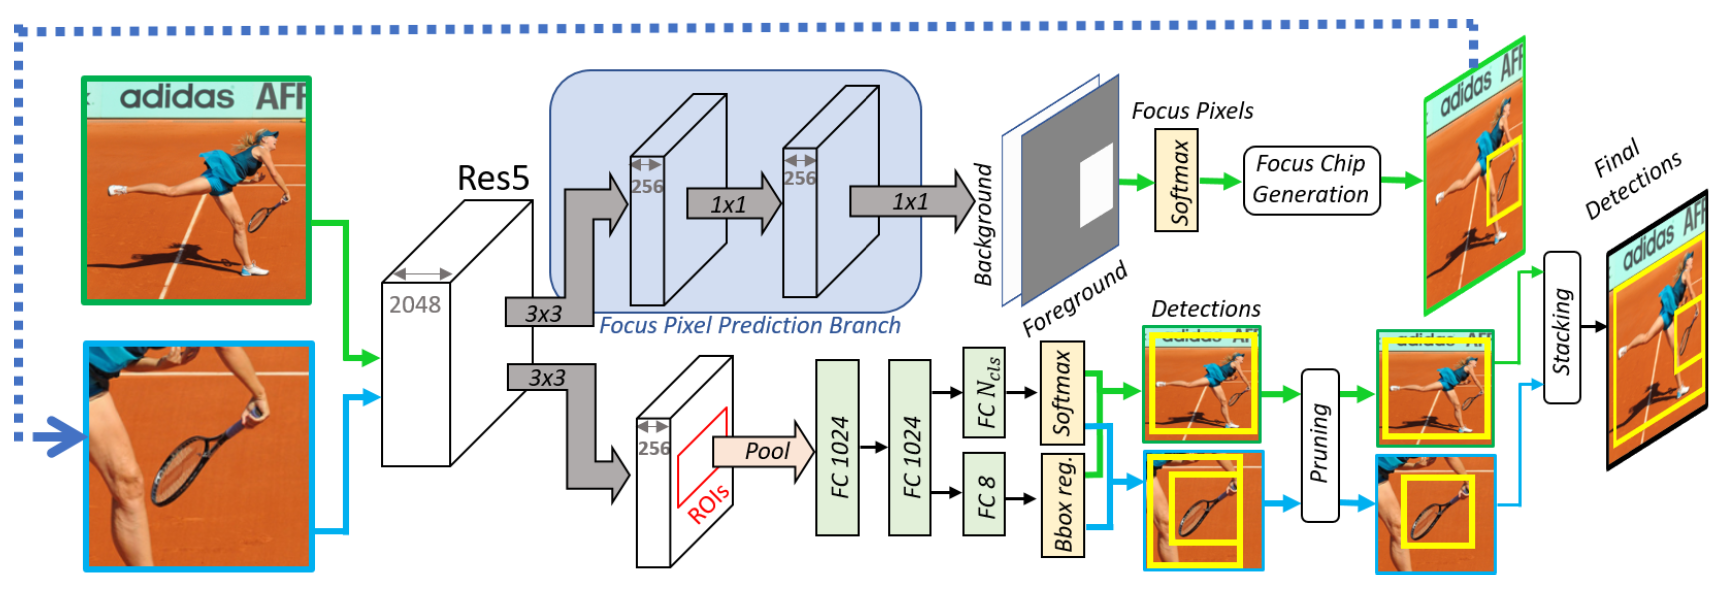
\includegraphics[width=15cm] {images/autofocus_model}
        \caption{Kiến trúc mô hình AutoFocus (Nguồn: \cite{najibi2019autofocus})}
        \label{fig:autofocus_model}
    \end{figure}
    
    \noindent
    Mô hình này nhận đầu vào xuất phát từ ảnh có kích thước nhỏ với mục tiêu định vị được những đối tượng có kích thước lớn và xác định khu vực khả năng cao chứa đối tượng.
    Với các khu vực khả năng cao chứa đối tượng, AutoFocus tiếp tục zoom vào với kích thước lớn hơn nhằm định vị được những đối tượng có kích thước nhỏ hơn và tiếp tục xác định khu vực khả năng cao chứa đối tượng.
    Quá trình này sẽ lặp đi lặp lại cho đến khi không còn khu vực nào cần phải zoom thì thuật toán sẽ dừng lại. \\
    Mô hình AutoFocus gồm ba thành phần là \textit{Thuật toán Focus Pixel} và \textit{Thuật toán sinh Focus Chips} thuộc nhánh Focus và \textit{Thuật toán Focus Stacking} thuộc nhánh Detection.

    \noindent
    \textbf{\textit{Thuật toán Focus Pixel}} \\
    Thuật toán Focus Pixel là thuật toán giúp chúng ta có thể xác định được vị trí khu vực có khả năng chứa đối tượng và cần zoom trên ảnh.
    Ý tưởng của thuật toán Focus Pixel dựa trên việc khi ta đưa đầu vào một ảnh có kích thước $X \times Y$ qua một khối Conv (như trong mô hình ResNet), feature maps mà ta thu được có kích thước $X' \times Y'$, trong đó: $X' = \lceil \frac{X}{s} \rceil$, $Y' = \lceil \frac{Y}{s} \rceil$, và $s$ là stride của cả khối Conv.
    Từ đó ta có thể ngầm hiểu rằng một pixel trên feature maps có kích thước $X' \times Y'$ đại diện cho một khu vực có kích thước $s \times s$ trên ảnh đầu vào. \\
    Với ý tưởng trên, từ groundtruth bounding box của đối tượng trên ảnh đầu vào, thuật toán Focus Pixel giúp xây dựng được label dạng mask của nhánh Focus với kích thước chiều dài chiều rộng bằng với khối Conv5 của mô hình backbone ResNet. \\
    Cụ thể hơn, Focus Pixel xác định các pixel trên mask là các \textit{pixel cần được focus} nếu như pixel đó có overlap với grountruth bounding box của đối tượng có kích thước nhỏ.
    Tiếp theo, các pixel trên mask là các \textit{pixel không cần quan tâm} nếu như pixel đó có overlap với groundtruth bounding box của đối tượng có kích thước lớn hoặc rất nhỏ.
    Cuối cùng, các \textit{pixel không cần được focus} trên mask là các pixel còn lại.

    \[l = 
        \begin{cases}
            1, & IoU(GT, l) > 0, a < \sqrt{GTArea} < b \\
            -1, & IoU(GT, l) > 0, \sqrt{GTArea} < a  \\
            -1, & IoU(GT, l) > 0, b < \sqrt{GTArea} < c  \\
            0, & \text{otherwise}
        \end{cases}
    \]

    \noindent
    trong đó: \\
    - $IoU(GT, l)$ là chỉ số IoU giữa khu vực $s \times s$ và groundtruth bounding box của đối tượng trên ảnh đầu vào. \\
    - $GTArea$ là diện tích của groundtruth bounding box của đối tượng trên ảnh đầu vào. \\
    Nếu một khu vực $s \times s$ overlap với nhiều groundtruth bounding box của đối tượng, thì pixel đó được ưu tiên là một Focus Pixel.

    \begin{figure}[H]
        \centering
        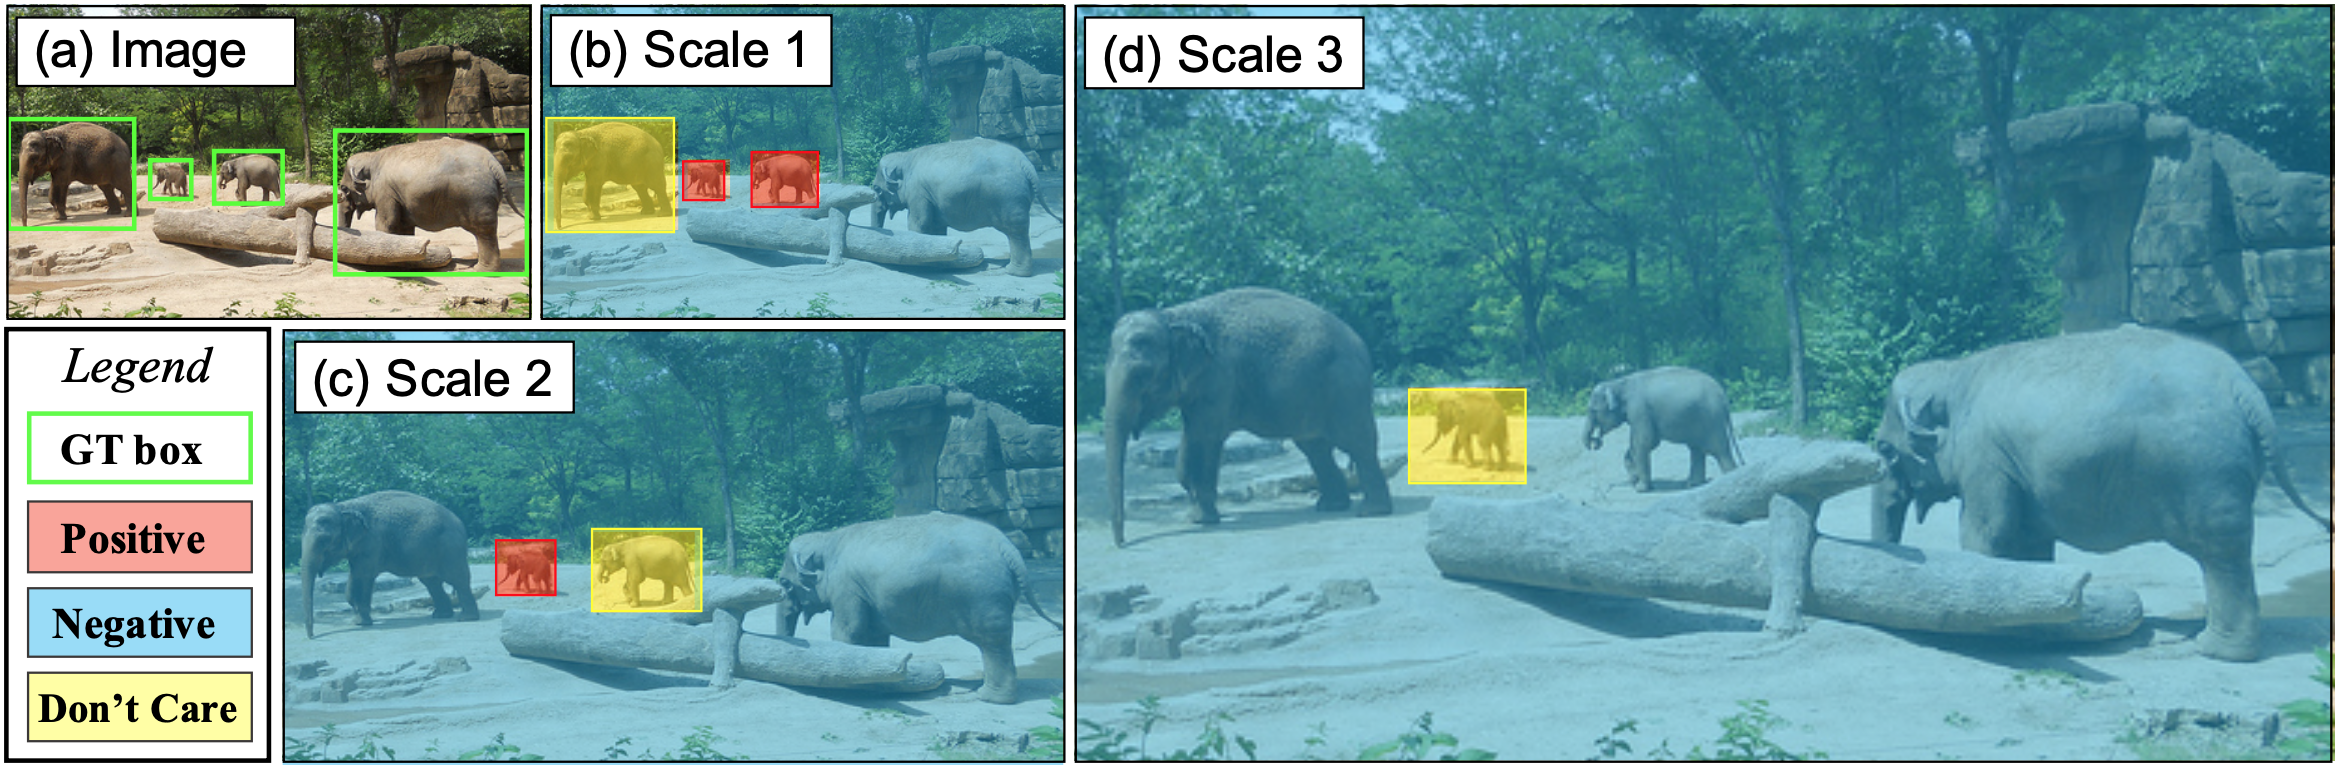
\includegraphics[width=15cm] {images/autofocus_focus_pixel}
        \caption{Ví dụ về cơ chế hoạt động của thuật toán Focus Pixel (Nguồn: \cite{najibi2019autofocus})}
        \label{fig:autofocus_focus_pixel}
    \end{figure}

    \noindent
    Trong các thí nghiệm mà nhóm tác giả thực hiện trong nghiên cứu, nhóm tác giả sử dụng ảnh đầu vào có kích thước $512 \times 512$, với các tham số $a = 5, b = 64, c = 90$ nghĩa là các groundtruth bounding box có kích thước từ $5 \times 5$ đến $64 \times 64$ là các bounding box cần được focus, các groundtruth bounding box có kích thước dưới $5 \times 5$ hoặc từ $64 \times 64$ đến $90 \times 90$ là các bounding box không cần quan tâm và các groundtruth bounding box có kích thước trên $90 \times 90$ là các bounding box không cần được focus.
    Từ các tham số trên, tỷ lệ giữa các \textit{pixel cần được focus} và \textit{pixel không cần được focus} là 10.

    \noindent
    \textbf{\textit{Thuật toán sinh Focus Chips}} \\
    Sau khi mô hình đã được train và predict ra được pixel cần được focus, mô hình cần một thuật toán để crop ra được khu vực cần focus trên ảnh làm đầu vào cho mô hình AutoFocus lượt tiếp theo.
    Và đó là vai trò của thuật toán sinh Focus Chips.

    \begin{figure}[H]
        \centering
        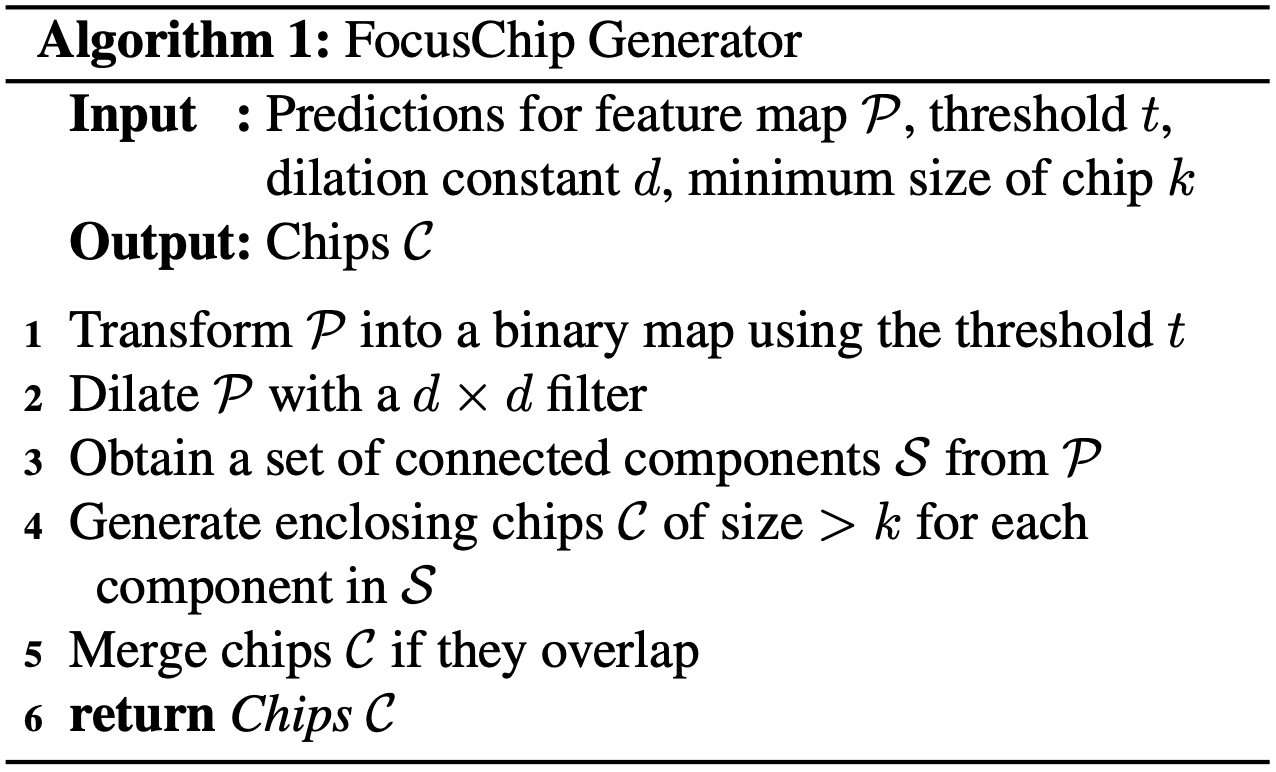
\includegraphics[width=10cm] {images/autofocus_focus_chip_gen}
        \caption{Chi tiết thuật toán sinh Focus Chips (Nguồn: \cite{najibi2019autofocus})}
        \label{fig:autofocus_focus_chip_gen}
    \end{figure}

    \noindent
    Trong quá trình predict, sau khi mô hình đã predict được các pixel cần được focus (ký hiệu là $\mathcal{P}$) trên Focus Pixel mask, ta biến đổi mask này trở về dạng binary mask bằng threshold $t$.
    Tham số $t$ được sử dụng để cân đối giữa tốc độ và độ chính xác của mô hình (cụ thể với tham số $t$ lớn, số lượng các pixel cần được focus sẽ giảm đi và tốc độ của mô hình AutoFocus sẽ tăng và ngược lại). \\
    Từ binary mask đã được sinh ra ở trên, thuật toán sinh Focus Chips sẽ đưa qua một filter có kích thước $d \times d$ nhằm giãn nở các pixel thêm một chút để thu được các thành phần liên thông $\mathcal{S}$, từ đó có nhiều thông tin hơn khi crop ảnh đầu vào với các focus pixel này. \\
    Cuối cùng, ta crop ra các chip $\mathcal{C}$ với kích thước tối thiểu là $k \times k$ và bao trọn các thành phần liên thông $\mathcal{S}$ trên.
    Các chip trong $\mathcal{C}$ nếu có overlap với nhau sẽ được gộp lại chung thành một chip. \\
    Việc sinh ra các chip $\mathcal{C}$ giúp mô hình AutoFocus có thể sử dụng ý tưởng Image Pyramids nhưng tiết kiệm chi phí tính toán nhờ loại bỏ các khu vực khả năng cao không chứa đối tượng.

    \noindent
    \textbf{\textit{Thuật toán Focus Stacking}} \\
    Một vấn đề cần phải giải quyết khi thực hiện predict với ý tưởng Image Pyramids trong bài toán object detection là việc tổng hợp lại các bounding box.
    Đối với mô hình AutoFocus, vấn đề này còn phức tạp hơn với trường hợp một đối tượng có kích thước lớn được dự đoán ở kích thước này, nhưng đến kích thước tiếp theo, đối tượng đó bị crop trong quá trình crop chip và trở thành một đối tượng có kích thước nhỏ hơn.
    Nhằm hạn chế bớt vấn đề này, nhóm tác giả chỉ ra rằng \textit{bước 2} trong thuật toán sinh Focus Chips \ref{fig:autofocus_focus_chip_gen} là cực kỳ quan trọng.

    \begin{figure}[H]
        \centering
        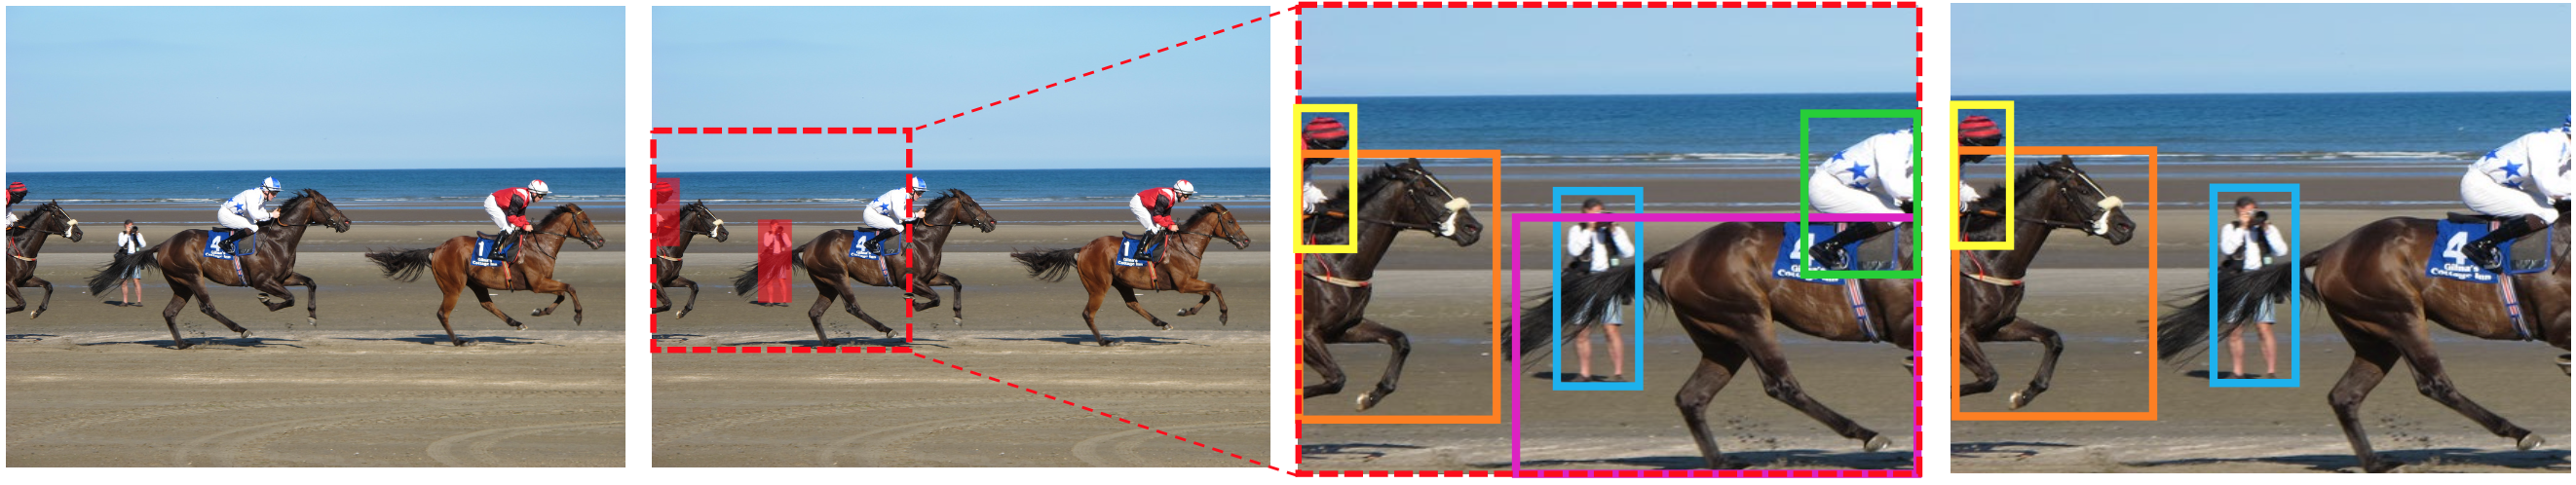
\includegraphics[width=10cm] {images/autofocus_focus_stack}
        \caption{Ví dụ về cơ chế hoạt động của thuật toán Focus Stacking (Nguồn: \cite{najibi2019autofocus})}
        \label{fig:autofocus_focus_stack}
    \end{figure}

    \noindent
    Tuy nhiên, nhóm tác giả cũng đề ra một số luật nhằm loại bỏ các dự đoán lỗi của các đối tượng được định vị trên một focus chip: \\
    - Nếu một đối tượng nằm trên một biên của chip nhưng không phải biên của ảnh đầu vào (nghĩa là đối tượng này đã bị crop sau khi qua thuật toán sinh Focus Chip), thì dự đoán sẽ bị loại bỏ. \\
    - Nếu một đối tượng nằm trên một biên của chip và đó là biên của ảnh đầu vào, nhóm tác giả sẽ tiếp tục kiểm tra biên còn lại của đối tượng, nếu đó là biên của chip, dự đoán sẽ bị loại, còn nếu đó không phải là biên của chip, dự đoán sẽ được giữ lại. \\
    - Nếu một đối tượng nằm trên hai biên của chip và đó đều là hai biên của ảnh đầu vào, nhóm tác giả sẽ giữ lại những dự đoán này. \\
    Sau khi loại bỏ bớt các dự đoán bằng thuật toán Focus Stacking, mô hình AutoFocus đưa ra tổng hợp dự đoán từ các kích thước ảnh khác nhau và là các dự đoán cuối cùng của ảnh đầu vào.

    \noindent
    \textbf{\textit{Kết quả của mô hình AutoFocus}} \\
    Kết quả của mô hình AutoFocus so sánh với các mô hình khác là rất ấn tượng trên bộ dữ liệu COCO test-dev.
    Số lượng pixel mà mô hình cần xử lý được chú thích tại cột \textit{Pixels}.
    Mô hình AutoFocus giữ được kết quả tương đương với mô hình sử dụng phương pháp chuẩn bị dữ liệu SNIPER trên tất cả các chỉ số trong khi đạt số lượng pixel cần xử lý ít hơn nhiều so với mô hình sử dụng SNIPER.

    \begin{figure}[H]
        \centering
        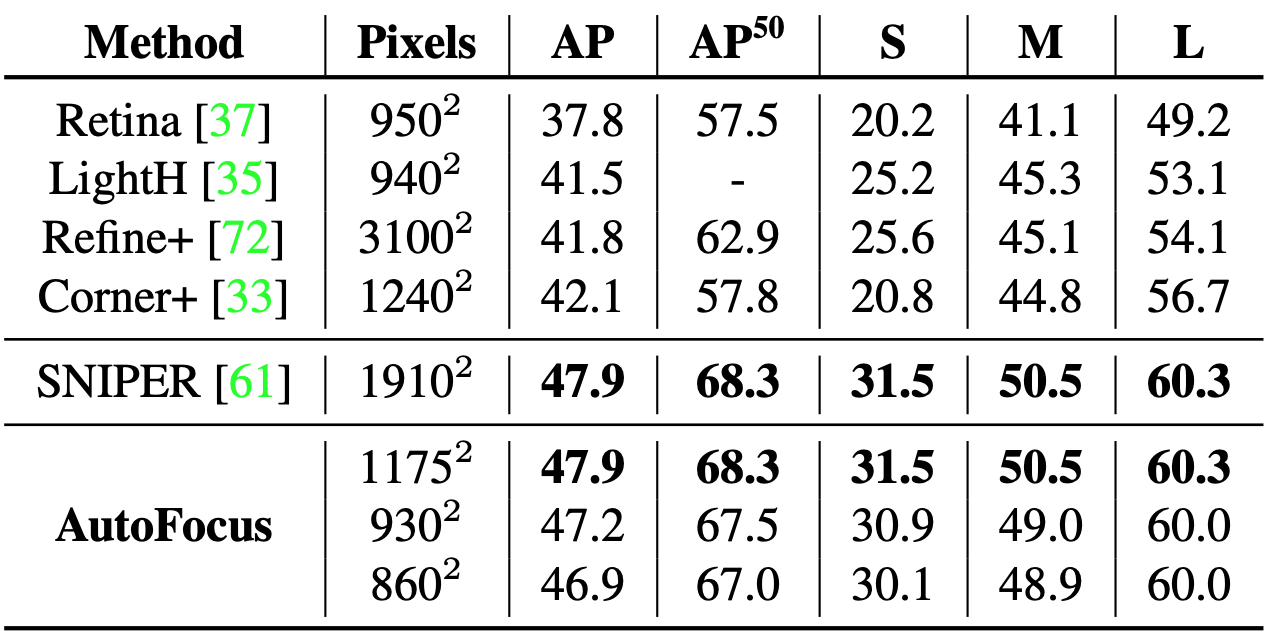
\includegraphics[width=10cm] {images/autofocus_results_1}
        \caption{Kết quả của mô hình AutoFocus so sánh với các mô hình khác trên bộ dữ liệu COCO test-dev (Nguồn: \cite{najibi2019autofocus})}
        \label{fig:autofocus_results_1}
    \end{figure}

    \noindent
    Nhóm tác giả chia sẻ rằng dù đạt kết quả là 47.9\% tương đương với SNIPER, nhưng AutoFocus có khả năng xử lý khoảng 6.4 ảnh/giây trên bộ COCO test-dev trên Titan X Pascal GPU so sánh với chỉ 2.5 ảnh/giây của mô hình sử dụng SNIPER. \\
    Mô hình RetinaNet với ResNet-101 backbone đạt tốc độ gần tương đương với AutoFocus là 6.4 ảnh/giây trên bộ COCO test-dev trên P100 GPU (tương đương với Titan X Pascal GPU) nhưng chỉ đạt mức mAP là 37.8\%.
    Nhóm tác giả cũng nhấn mạnh rằng AutoFocus là mô hình nhanh nhất ở thời điểm đó xử lý bộ dữ liệu COCO và đạt chỉ số mAP là 47.9\%.

    \begin{figure}[H]
        \centering
        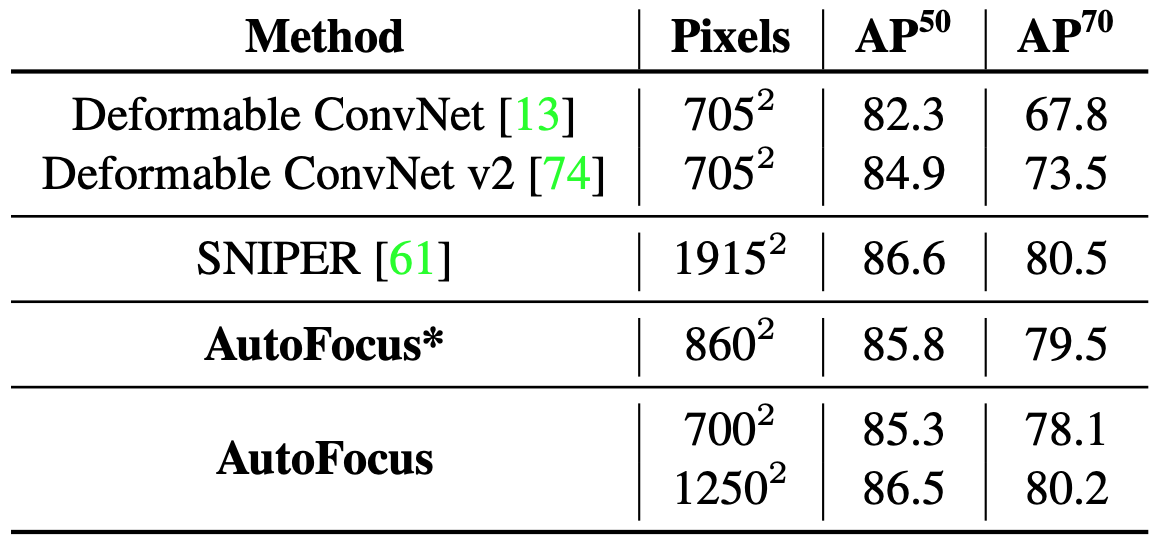
\includegraphics[width=10cm] {images/autofocus_results_2}
        \caption{Kết quả của mô hình AutoFocus so sánh với các mô hình khác trên bộ dữ liệu PASCAL VOC 2007 test-set (Nguồn: \cite{najibi2019autofocus})}
        \label{fig:autofocus_results_2}
    \end{figure}

    \noindent
    Kết quả của mô hình AutoFocus so sánh với các mô hình khác trên bộ dữ liệu PASCAL VOC 2007 test-set cũng được nhóm tác giả chia sẻ.
    Ở đây, nhóm tác giả cũng nhấn mạnh vào sức mạnh của mô hình AutoFocus khi sử dụng cấu hình được finetune của mô hình trên bộ dữ liệu COCO (mô hình ký hiệu là AutoFocus*) để giải quyết bộ dữ liệu PASCAL VOC 2007 nhưng vẫn đạt kết quả tốt.

    \begin{figure}[H]
        \centering
        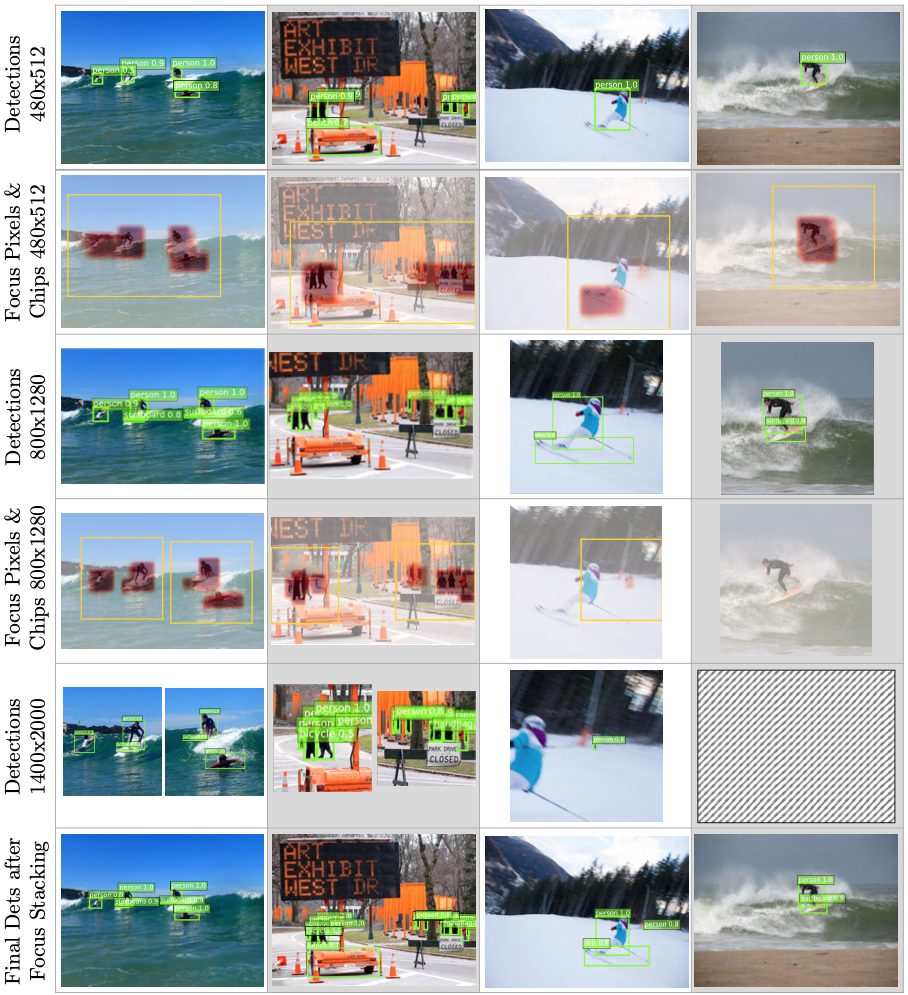
\includegraphics[width=10cm] {images/autofocus_results_3}
        \caption{Từng bước quá trình dự đoán của mô hình AutoFocus với một số ảnh trong bộ dữ liệu COCO val-2017(Nguồn: \cite{najibi2019autofocus})}
        \label{fig:autofocus_results_3}
    \end{figure}

    \noindent
    \textbf{\textit{Vấn đề tồn đọng của mô hình AutoFocus}} \\
    Nghiên cứu của mô hình AutoFocus đã mang lại một ý tưởng rất thông minh để xử lý rất nhanh bài toán object detection với ảnh chất lượng cao trong khi vẫn duy trì được độ chính xác cao, tương đương với các mô hình sử dụng phương pháp Image Pyramids truyền thống.
    Tuy nhiên, mô hình AutoFocus vẫn tồn tại điểm yếu khá lớn là số lượng hyperpameter của mô hình nhiều.
    Điều này gây ra khó khăn trong việc tìm kiếm một cấu hình tốt nhất của mô hình đối với từng bài toán hay từng bộ dữ liệu khác nhau.
    Nghiên cứu và phân tích về điểm yếu này sẽ được trình bày trong phần sau của luận văn.
}